\section{Constraints}

Modelling is the field of formalising assumptions about the world in logical and mathematical terms.
The formality of such models allows us to test, validate and analyse our model using objective, rather than subjective observations.
However, the more assumptions we make, the more specific our model is.
Perhaps it even makes our model less useful, because it is too specific.
Conversely, the less assumptions we make, the more general our model is.
But implicitly, it is more difficult to model (as there are more variables to capture).\\
\\
As we are building a (formal) model for defect detection and fixing, it is implicit that we too will make assumptions that we encode into our model.
It is thus worthwhile to discuss our observations and assumptions.
More importantly, we ought to justify why assumptions could be made and what their impact on the results are.\\
\\
This chapter begins by describing our problem, in terms of observations and open questions.
We then lay down our assumptions to answer the open questions, as well as justifications for {\em why} these assumptions were made.
We summarise our results in our final subchapter.

\subsection{Observations}

We will lay down our model assumptions by first describing the data we are working with.
We are given data about a two-stage process which finds, then fixes defects.
This project involves 3 software engineers who worked 25 hours per week, where one engineer was testing.
The data provided is the result of that engineer devoting all of his/her time to testing each
week and uncovering defects.\\
\\
Defects can be classed into 2 levels of ``severity", and 2 levels of "difficulty".
They are of either \major or \minor severity, and either \easy or \hard in terms of difficulty.
We are told that \major defects are approximately ``seven times as damaging on average as minor
ones".
Furthermore, on average a \hard defect requires 5 hours to fix, whilst an \easy defect requires 2
hours to fix \cite{duterryassspeci}.
We shall take on the role of the project manager and use models to simulate different strategies against different
metrics.\\
\\
This describes the data and initial constraints of our model.
There are many open questions that we ought to at least consider, and hopefully answer before
beginning our modelling.
We enumerate them below
\begin{enumerate}
	\item can an engineer do ``part of" a defect?
	For example, if an engineer has 1 hour left in their working week, can they do half of an \easy
defect? \label{openQuestOne}
	\item we have estimated the ``impact" --- how does this translate to impacting the customer?
	Is it by money?
	By time?
	Should we assign some units to it, or is the arbitrary ``severity" measure good enough?
	\label{openQuestTwo}
	\item are our estimates of ``severity" and ``difficulty" accurate?
	If they are not, how accurate are they actually, and how does inaccuracy translate in our model?
	\label{openQuestThree}
	\item when do defects get fixed?
	In real life, the defect detection/fixing process is a two-stage parallel process, where detection
puts defects onto an ordered priority queue of defects to fix, whilst fixing simultaneously takes
defects from the priority queue for fixing.
	This is illustrated in Figure \ref{realDefectProcess}. \label{openQuestFour}
	\item does the testing engineer only do testing?
	Can they do other work?
	Are they as effective at doing other work? \label{openQuestFive}
	\item if a testing engineer can do other work, when do they stop testing and start other work?
	And when do they become a testing engineer again? these questions apply equally to a normal software engineer and we ought to answer them for
the development engineers \label{openQuestSix}. 
	\item are defects independent of each other? Do they have no dependencies? \label{openQuestSeven}
	\item when a defect is fixed, does it reintroduce bugs or is it always fixed?
	\label{openQuestEight}
	\item if we had twice as many testers, would we go through our defect detection data twice as
quickly? \label{openQuestNine}
	\item does a defect only affect the customers the moment the tester has found them?
	Indeed, is the tester the only way of a defect to be detected? \label{openQuestTen}
	\item what do we actually want to measure? \label{openQuestEleven}
	\item will the severity or difficulty of defects ever change? \label{openQuestTwelve}
  \item are there defects we do not want to fix? \label{openQuestThirteen}
\end{enumerate}

\begin{figure}[ht!]
  \centering
	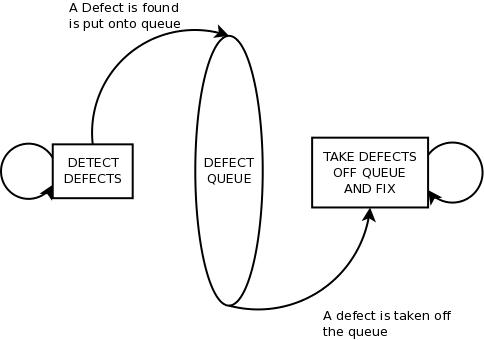
\includegraphics[scale=0.5]{Blah.png}
	\caption{The usual way a defect detection-fixing process works.
  Each is an independent process that works in parallel.} \label{realDefectProcess}
\end{figure}

We will now outline and justify our assumptions, and answer the open questions we have raised as
best we can.

\subsection{Assumptions about our simulation}

Firstly, Question \ref{openQuestOne} asks whether we can have ``part fixes".
We will disallow this in our simulation --- it makes the model more realisitc but at this stage it
is too difficult to model.
For Question \ref{openQuestTwo} we will simply let the model measure severity in its
unitless form --- there is less to be gained from attaching some unit to it since we have no concept
of what our client values and how they are being affected here.\\
\\
For Question \ref{openQuestThree}, we are going to assume the estimates are exactly accurate.
This is, of course, a blatant falsehood --- there are estimation techniques such
as \cite{pulford1996overconfidence} which
indicate the {\em confidence} of an estimate.
Indeed, estimates are seemingly useless without some idea of standard deviation or variance.
Nevertheless, for ease of modelling we will let the values for \easy, \hard, \minor and \major be
exact values of the difficulty and severity of fixing a defect.\\
\\
Question \ref{openQuestFour} again opens a method by which the accuracy of our model, and its power
could be much improved.
If the defect fixing and detection process actually resembles Figure \ref{realDefectProcess}, our
model would be quite an accurate representation of the real world.
This is difficult to actually build into our model, however.
For the purposes of this paper, we limit our model to a sequential, instead of parallel defect
detection and fixing process.
This process is shown in Figure \ref{fakeDefectProcess}.

\begin{figure}[ht!]
  \centering
	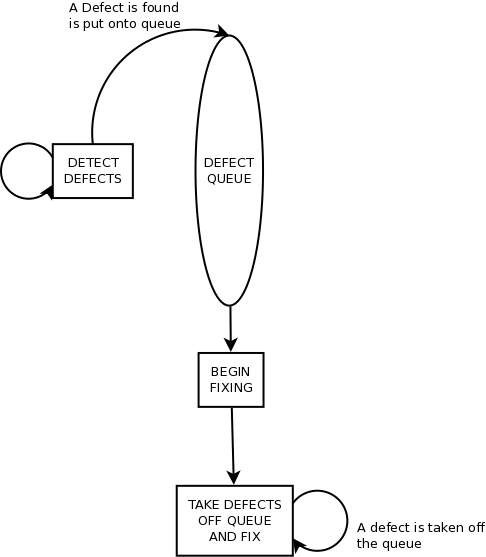
\includegraphics[scale=0.5]{Derp.png}
	\caption{ Our way of modelling a process. In this case, this is a serial
    process, that is it is sequential. We fill the queue in the detection
      process, then pass it to the fixing process. It it not an accurate reflection, but it
  is easier to model.} \label{fakeDefectProcess}
\end{figure}

Questions \ref{openQuestFive} and \ref{openQuestSix} ask whether a software engineer should be reassigned from testing, and
when that should occur.
We will allow this, and its occurrance is something we are interested in.
How should we allocate resources?
When should we do so?
These are artefacts of the strategies we use, and the simulation will allow a strategy to test
this.
We will also say that all software engineers are equally competent at testing and development,
although it is true, as from tutorials that some engineers might be approximately twenty times
more skilled than another engineer.\\
\\
To make our modelling easier, we assume that for Question \ref{openQuestSeven} all defects are
independent and do not affect each other.
This is not a good reflection of the world (in my opinion, which I would say is
    logically sound but I cannot qualify with references at this stage) but it makes our modelling process much
easier since we need not construct some topological order which defects should be fixed in.\\
\\
We say for Question \ref{openQuestEight} that a defect will not reintroduce bugs into our system.
For Question \ref{openQuestNine} we claim that this is indeed the case, and if we assign more people
to testing then the effect scales multiplicatively.
Conversely, the fewer people in testing, the slower defect detection will be.
People also cannot split their time between defect detection and defect fixing --- they are either
doing one or the other the whole time.
Of course, all of this is not an accurate reflection of the real world (indeed, Brooks espouses in
\ref{brooks1987no} why the assumption of more people speeding up software work is particularly flawed), but again
it eases the modelling process.\\
\\
We say that for Question \ref{openQuestTen}, the only person finding defects are the
testers.
Implicitly, a developer can only fix a defect after a tester has found it.
This element of randomness from users is much more difficult to model (we theorise that it could be
done with a Poisson distribution) and so we will assume it cannot occur.\\
\\
Perhaps an odd question is \ref{openQuestThirteen} --- why would we {\em not}
want to fix a defect?
We will assume that all defects must be fixed, but it is a fair question.
Is the defect actually a defect?
Is it someone not reporting correctly, or is it a duplicate?
Perhaps the workaround is already so ingrained into the users that it causes
more trouble to remove it!
Finally, and again for the sake of ease of modelling Question \ref{openQuestTwelve}, defects cannot
change their severity or their difficulty.
Once detected their attributes will remain the same.

\subsection{What are we measuring?}

To answer Question \ref{openQuestEleven}, we must also give thought to 
\begin{itemize}
	\item what we are measuring
	\item assumptions about how the client behaves and
	\item what interests both us and them.
\end{itemize}

To begin with, let us discuss the tangential topic of ``internal" and ``external"
perspectives on a project.
I will say that a software engineering project has two views --- the ``internal" view, which is
that of a software organision, and the ``external" view, which is that of a
client (this is qualified in references within our lectures, but unfortunately I
    do not have the references).
We want to be able to model our process in terms of these metrics, to gauge the client's view of our
efforts, and also make useful measurements for our own ``internal" usage.
Note that this does {\em not} mean that an ``external" metric is not useful for the ``internal"
metrics --- rather, we say that ``internal" metrics measure things that are less desired or useful
to the client than an ``external" metric.\\
\\
We will make the following assumptions about the client behaviour
\begin{itemize}
	\item clients prefer major defects to be fixed over minor defects --- this seems logical since a
client is being affected negatively seven times more by a major defect, than by a minor one
	\item clients prefer defects to be fixed quickly --- this is evidenced by
  \cite{gaugingStakeholderPerc}
\end{itemize}

We will aim to measure the following ``external" metrics
\begin{itemize}
	\item queue severity --- a simple sum that takes into the total importance of found defects yet to
be fixed.
	Note that it does not increase the severity for defects that have been in the queue for longer ---
according to \cite{gaugingStakeholderPerc} this degrades client satisfaction and it was actually an oversight of my
modelling process to not do this.
	\item on average, how long have major defects been within the queue?
	This is related to our above comments on the importance of timeliness of fixes and the perception
that slow fixes has on clients, as shown in \cite{gaugingStakeholderPerc}
  \item the estimated number of major defects remaining in the system, an important estimate to a
client
	\item the ratio of major defects to major defects found in that week
\end{itemize}

We will also measure the following ``internal" metrics
\begin{itemize}
	\item the estimated number of defects remaining, no matter what severity or difficulty they are
--- this will give us a stopping criteria.
	We will assume that an exponential line of best fit can be fitted to the data, using a model
similar to Boehm's COCOMO equations \cite{boehm1984software}.
	We thus expect that the number of defects remaining in a system can be modelled by a negative
exponential, as in Figure \ref{negExp}.
	\item the size of our defect queue --- indeed, this is a metric that could be used in an audit,
though whether such a measurement is appopriate for an audit of our processes or teams is another
unrelated matter
	\item the average time a defect has been in our defect queue
	\item the ratio of defects fixed to defects found in that week
\end{itemize}

\begin{figure}[ht!]
  \centering
  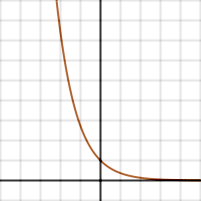
\includegraphics[scale=0.75]{Exp.png}
	\caption{A sample negative exponential function. This is how I expect the
    model will behave with respect to number of defects remaining in the system
      \cite{negex}.} \label{negExp}
\end{figure}

\subsection{Summary of metrics and assumptions}

In summary, we make the following assumptions:
\begin{itemize}
	\item no partial fixes
	\item unitless severity
	\item all estimates are reliable and entirely accurate
	\item sequential, as opposed to parallelised defect fixing process
	\item engineers can be reassigned --- an artefact of the strategy
	\item engineers are all equally competent at all tasks, whether it is testing or development
	\item defects are independent and do not have an ordering that must be adhered to when fixing them
	\item defect fixing does not reintroduce defects
	\item having $k$ testers implies we will complete our work $k$ times as quickly
	\item only the tester is finding the defects, and developers cannot fix a defect unless a tester
has found it
  \item we want to remove all defects we find
	\item a defect is immutable, in the sense that once its severity and difficulty are established
they can neither escalate nor be downplayed
\end{itemize}

These assumptions seem, perhaps, to be very trivial or to not reflect the actual state of a software
engineering project.
The observant reader will note that the reasons for most of these assumptions are ``they make the modelling
process easier".
It is unfortunate that these notions cannot at this stage be challeneged, but we will give a
treatise later on how we might challenge or improve our models.\\
\\
We will measure the following ``external" metrics
\begin{itemize}
	\item queue severity
	\item the average amount of time, in weeks, that a major defect is in the queue
	\item the estimated number of major defects remaining in the system
	\item the ratio of major defects to major defects found in that week
\end{itemize}

We will also measure the following ``internal" metrics.
\begin{itemize}
	\item the estimated number of defects remaining
	\item the size of our defect queue
	\item the average time, in weeks, that a defect has been in our defect queue
	\item the ratio of defects fixed to defects found in that week
\end{itemize}
